\documentclass[12pt]{article}
\usepackage[utf8]{inputenc}
\usepackage[automark]{scrlayer-scrpage}
\usepackage[T1]{fontenc}
\usepackage[pdftex]{graphicx,color}
\usepackage{subcaption}
\usepackage{url}
\usepackage[pdftex,pdfpagelabels]{hyperref}
\usepackage[section,boxed]{algorithm}
\usepackage{algpseudocode}
\usepackage{amsmath}
\usepackage{amssymb}
\usepackage{amsthm}
\usepackage{lmodern}
\pagestyle{scrheadings}
\ofoot{}\cfoot{}\ifoot{}
\lehead{\pagemark}
\rehead{\slshape\leftmark}
\lohead{\slshape\leftmark}
\rohead{\pagemark}
\newtheorem{definition}{Definition}
\newtheorem{theorem}{Theorem}
\usepackage{blindtext}
\usepackage[ngerman]{babel}
\usepackage[margin=1in]{geometry}
\usepackage{amsmath,amsthm,amssymb}
\usepackage{graphicx}
\usepackage{svg}
\newcommand{\N}{\mathbb{N}}
\newcommand{\Z}{\mathbb{Z}}
\newcommand{\R}{\mathbb{R}}
\newcommand{\C}{\mathbb{C}}

\begin{document}
% --------------------------------------------------------------
%                         Title Page
% --------------------------------------------------------------
\title{Solutions for Sheet 4}
\author{Raphael Wude, Martin Brückmann, Claude Jordan, Daniel Degenstein\\ \\
\textsc{Pattern Matching and Machine Learning} \\
\textsc{for Audio Signal Processing}}
\maketitle

% --------------------------------------------------------------
%                         Task 4.1
% --------------------------------------------------------------
\section*{Task 4.1}
\subsection*{(a)}
$X_{0}=(\omega^{0\cdot0}_{N},...,\omega^{0\cdot(N-1)}_{N})\cdot x$\\\\
$=\sum^{N-1}_{k=0} \omega^{0}_{N}\cdot x_{k}$\\\\
$=\sum^{N-1}_{k=0} x_{k} ~~~\Rightarrow X_{0} \in \mathbb{R}$\\\\\\
$X_{M}=(\omega^{0\cdot M}_{N},...,\omega^{(N-1)\cdot M}_{N})\cdot x$\\\\
$=\sum^{N-1}_{k=0} \omega^{kM}_{N}\cdot x_{k}$\\\\
$=\sum^{N-1}_{k=0} exp(\frac{-2\pi iM}{N})^{k}\cdot x_{k}$\\\\
$=\sum^{N-1}_{k=0} exp(\frac{-2\pi iMk}{2M})\cdot x_{k}$\\\\
$=\sum^{N-1}_{k=0} exp(-\pi ik)\cdot x_{k}$\\\\
$=\sum^{N-1}_{k=0} (-1)^{k}\cdot x_{k} ~~~\Rightarrow X_{M} \in \mathbb{R}$\\\\\\
$X_{N-k}=\sum^{N-1}_{l=0} \omega^{l(N-k)}_{N}\cdot x_{l}$\\\\
$=\sum^{N-1}_{l=0} exp(\frac{-2\pi il(N-k)}{N})\cdot x_{l}$\\\\
$=\sum^{N-1}_{l=0} exp(\frac{-2\pi ilN}{N}-(\frac{-2\pi ilk}{N}))\cdot x_{l}$\\\\
$=\sum^{N-1}_{l=0} exp(\frac{2\pi ilk}{N}-2\pi ilN)\cdot x_{l}$\\\\
$=\sum^{N-1}_{l=0} exp(\frac{2\pi ilk}{N})\cdot exp(-2\pi ilN)\cdot x_{l}$\\\\
$=\sum^{N-1}_{l=0} exp(\frac{2\pi ilk}{N})\cdot x_{l}$\\\\
$=\overline{\sum^{N-1}_{l=0} exp(\frac{-2\pi ilk}{N})\cdot x_{l}}$\\\\
$=\overline{\sum^{N-1}_{l=0} \omega^{lk}_{N}\cdot x_{l}}$\\\\
$=\overline{X_{k}}$

\subsection*{(b)}


\section*{Task 4.2}
\subsection*{(a)}
For A we got:
\begin{align*}
A = \text{DFT}_N \cdot a = \text{DFT}_N \cdot \left(sin\left(\frac{2\pi 4 k}{N}\right) \right)
\end{align*}
And with Eulers Formula:
\begin{align*}
  a &= sin\left(\frac{2\pi 4 k}{N}\right) = \frac{1}{2i} \cdot \left(e^{\frac{2\pi 4 ki}{N}}-e^{\frac{- 2\pi 4 ki}{N}}\right)\\
  &= \frac{1}{2i} \cdot (u_4 - u_{N-4})
\end{align*}
With $\langle u_k|u_l \rangle =N \cdot \delta_{k,l}$ we get:
\begin{align*}
  |a(k)| = \frac{N}{2} \cdot w_k
\end{align*}
with $w_4 = w_{N-4} = 1$ and else $w_k=0$.\\
That means, for $A= \text{DFT}_N \cdot a$ the only nonzero entries of the matrix A are at $k=4$ and $k=N-4=508$. For this entries we get:
\begin{align*}
  A(k) = \text{DFT}_N(k) \cdot \frac{N}{2}
\end{align*}

\subsection*{(b)}
We know, that $|A(k)|> 2 \theta$ for all nonzero $A(k)$ and $R(k)\leq \theta$. So $|A+R|>\theta$ for all $k\in \{0,...,N-1\}$. So for $B_\theta$ we get:
\begin{align*}
  B_{\theta}(k) = \big\{ \begin{array}{l} A(k) + R(k), \text{for} k=4 \wedge k=508 \\ 0, \text{else} \end{array}
\end{align*}
If we now define us a new $R_\theta$ with:
\begin{align*}
  R_{\theta}(k) = \big\{ \begin{array}{l} R(k), \text{for} k=4 \wedge k=508 \\ 0, \text{else} \end{array}
\end{align*}
we can write $B_\theta=A + R_\theta$\\
So for $\tilde{a}$ and $\tilde{a}-a$  we get:
\begin{align*}
  \tilde{a} &= \text{DFT}_n^{-1} B_\theta = \text{DFT}_n^{-1} (A + R_\theta) = \text{DFT}_n^{-1} A + \text{DFT}_n^{-1} R_\theta = a + \text{DFT}_n^{-1} R_\theta \\
  \tilde{a}-a &= a + \text{DFT}_n^{-1} R_\theta - a = \text{DFT}_n^{-1} R_\theta
\end{align*}

\section*{Task 4.3}

\begin{figure}[h]\begin{figure}[h]
          \centering
          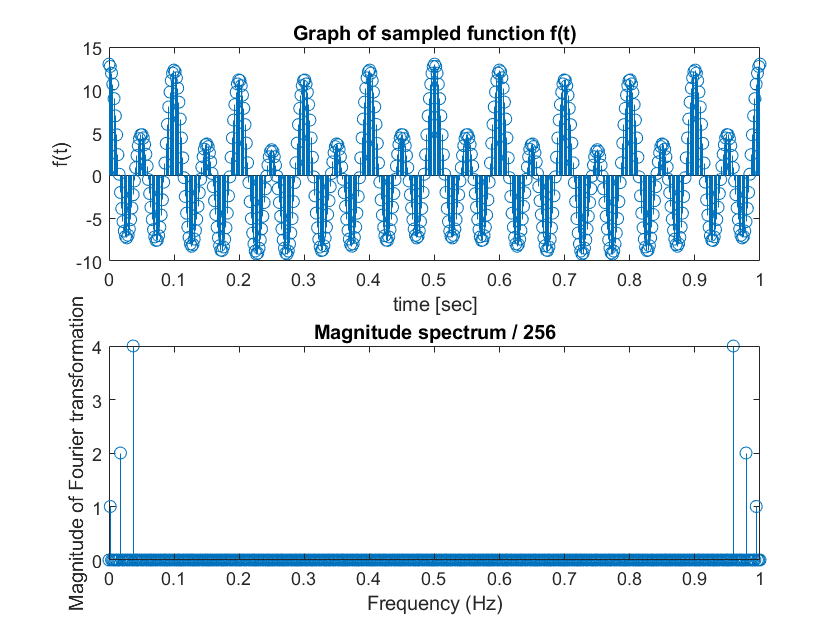
\includegraphics[width=1.1\textwidth]{Sheet3Exercise1.png}
          \caption{$f(t) \text{(top) and} |\hat f(k)| \text{(bottom)}$}
          \label{abb}
      \end{figure}
    \centering
    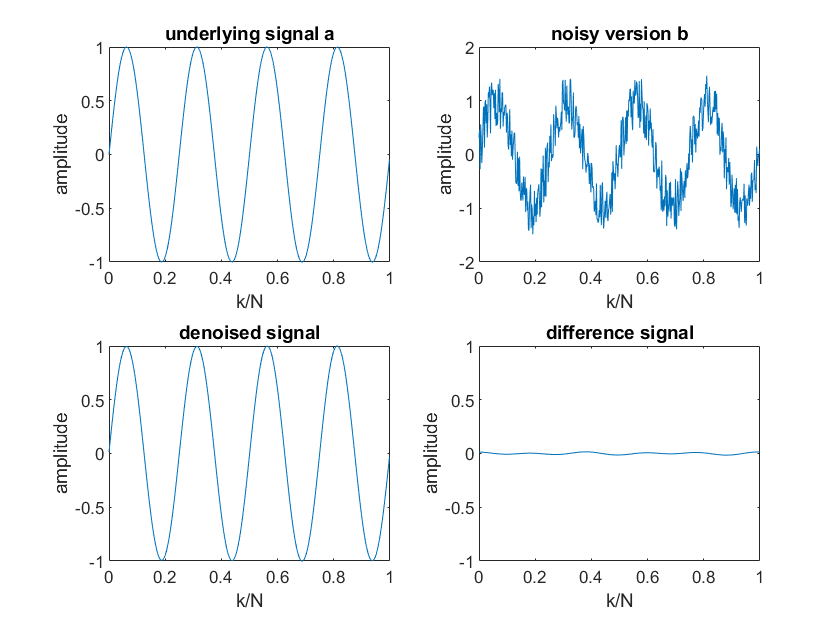
\includegraphics[width=1.1\textwidth]{ex3.png}
    \label{abb}
\end{figure}

\end{document}
